% Fig. 1 revision: larger label fonts, label clearance, r_u label.
% Fig. 1 (integrated, wide): scalable shared embedding transceiver in
% one left-to-right chain, with the periodic unit-codebook construction
% embedded in the transmitter and the directly scaled full codebook
% shown as the replaced alternative.
% Compile standalone:  latexmk fig1_integrated_revision.tex  (from project root),
% move out/fig1_integrated_revision.pdf to fig/, delete byproducts from out/.
\documentclass[tikz,border=2pt]{standalone}
\usepackage{amsmath,amssymb,bm}
\usetikzlibrary{arrows.meta,positioning,calc,fit,decorations.pathreplacing}
\begin{document}
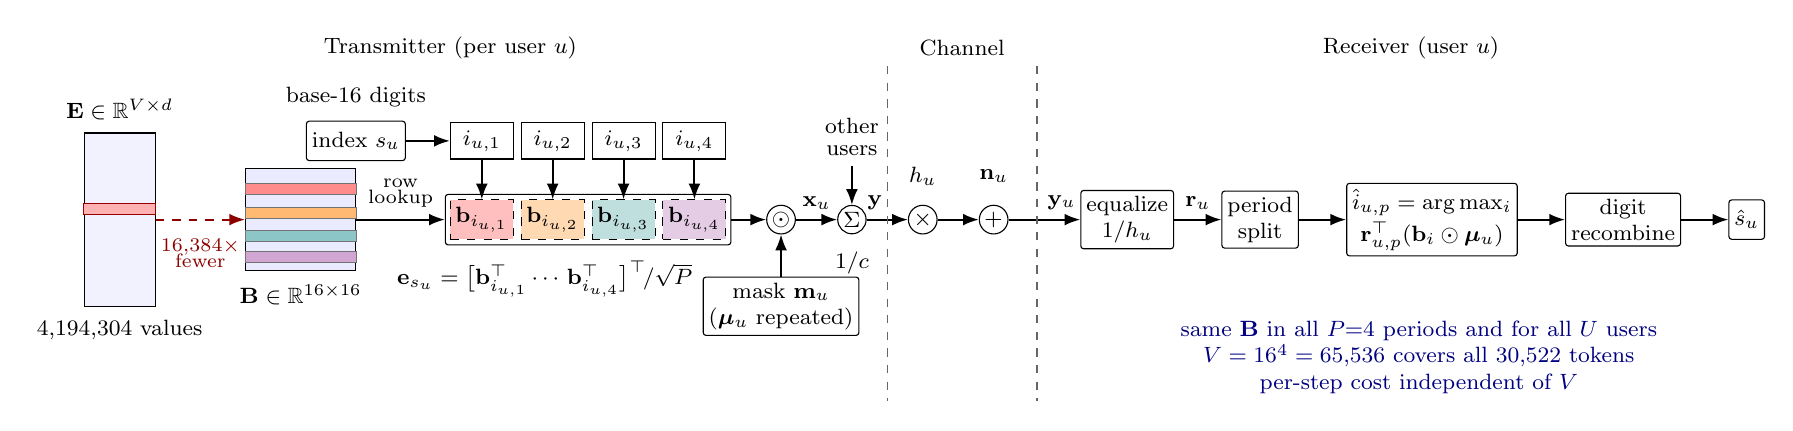
\begin{tikzpicture}[
  font=\footnotesize,
  lbl/.style={font=\footnotesize},
  ar/.style={-{Latex[length=2.0mm,width=1.5mm]},line width=0.7pt},
  blk/.style={draw,rounded corners=1pt,minimum height=5mm,inner sep=2pt,
              align=center},
  op/.style={draw,circle,inner sep=0.6pt,minimum size=3.6mm},
  dig/.style={draw,minimum width=8mm,minimum height=4.6mm,inner sep=1pt},
  seg/.style={draw,dashed,thin,minimum width=8mm,minimum height=5mm,
              inner sep=1pt},
  brc/.style={decorate,decoration={brace,mirror,amplitude=1.8mm}}
]

% ---------------- replaced full codebook (far left) ----------------
\node[draw,fill=blue!5,minimum width=9mm,minimum height=22mm]
  (E) at (-0.5,0) {};
\draw[fill=red!30,draw=red!60!black]
  ($(E.north west)+(0,-9mm)$) rectangle ($(E.north east)+(0,-10.4mm)$);
\node[lbl,anchor=south] (Etop) at ($(E.north)+(0,0.04)$)
  {$\mathbf{E}\in\mathbb{R}^{V\times d}$};
\node[lbl,anchor=north] (Ebot) at ($(E.south)+(0,-0.05)$)
  {$4{,}194{,}304$ values};

% ---------------- unit codebook ----------------
\node[draw,fill=blue!8,minimum width=14mm,minimum height=13mm]
  (B) at (1.8,0) {};
\foreach \y/\c in {2.0/red!45,5.0/orange!55,8.0/teal!45,10.6/violet!35}{
  \draw[fill=\c,draw=black!55]
    ($(B.north west)+(0,-\y mm)$) rectangle ($(B.north east)+(0,-\y mm-1.4mm)$);
}
\node[lbl,align=center,anchor=north] (Bbot) at ($(B.south)+(0,-0.05)$)
  {$\mathbf{B}\in\mathbb{R}^{16\times16}$};
\draw[ar,dashed,red!55!black] (E.east) --
  node[font=\scriptsize,below=1.2mm,text=red!55!black,align=center]
  {$16{,}384\times$\\[-0.3em]fewer} (B.west);

% ---------------- digit row above the frame ----------------
\node[blk] (idx) at (2.5,1.0) {index $s_u$};
\node[dig] (d1) at (4.1,1.0) {$i_{u,1}$};
\node[dig] (d2) at (5.0,1.0) {$i_{u,2}$};
\node[dig] (d3) at (5.9,1.0) {$i_{u,3}$};
\node[dig] (d4) at (6.8,1.0) {$i_{u,4}$};
\draw[ar] (idx.east) -- (d1.west);
\node[lbl,anchor=south] at ($(idx.north)+(0,0.05)$) {base-$16$ digits};

% ---------------- embedding frame ----------------
\node[seg,fill=red!25]    (s1) at (4.1,0) {$\mathbf{b}_{i_{u,1}}$};
\node[seg,fill=orange!30] (s2) at (5.0,0) {$\mathbf{b}_{i_{u,2}}$};
\node[seg,fill=teal!25]   (s3) at (5.9,0) {$\mathbf{b}_{i_{u,3}}$};
\node[seg,fill=violet!20] (s4) at (6.8,0) {$\mathbf{b}_{i_{u,4}}$};
\foreach \k in {1,2,3,4}{\draw[ar] (d\k.south) -- (s\k.north);}
\node[draw,rounded corners=1pt,inner xsep=1.6pt,
      inner ysep=1.8pt,fit={(s1)(s4)}] (frame) {};
\draw[ar] (B.east) -- node[font=\scriptsize,above=0.3mm,align=center,pos=0.5]
  {row\\[-0.3em]lookup} (frame.west);
\node[lbl,anchor=north] at (4.9,-0.4)
  {$\mathbf{e}_{s_u}=\big[\mathbf{b}_{i_{u,1}}^{\top}\cdots\,\mathbf{b}_{i_{u,4}}^{\top}\big]^{\top}\!/\sqrt{P}$};

% ---------------- superposition and channel ----------------
\node[op] (mul) at (7.9,0) {$\odot$};
\node[blk] (mask) at (7.9,-1.1)
  {mask $\mathbf{m}_u$\\($\bm{\mu}_u$ repeated)};
\node[op] (sum) at (8.8,0) {$\Sigma$};
\node[op] (ch)  at (9.7,0) {$\times$};
\node[op] (noise) at (10.6,0) {$+$};
\node[lbl] at (9.7,0.55) {$h_u$};
\node[lbl] at (10.6,0.55) {$\mathbf{n}_u$};
\node[lbl] at (8.8,-0.55) {$1/c$};
\draw[ar] (frame.east) -- (mul.west);
\draw[ar] (mask.north) -- (mul.south);
\draw[ar] (mul) -- node[lbl,above]{$\mathbf{x}_u$} (sum);
\draw[ar] ($(sum.north)+(0,0.5)$) node[lbl,above,align=center]
  {other\\[-0.2em]users} -- (sum.north);
\draw[ar] (sum) -- node[lbl,above,pos=0.2]{$\mathbf{y}$} (ch);
\draw[ar] (ch) -- (noise);

% ---------------- receiver (same row, to the right) ----------------
\node[blk,anchor=west] (eq) at (11.7,0) {equalize\\$1/h_u$};
\node[blk,right=6mm of eq] (ps) {period\\split};
\node[blk,right=6mm of ps] (corr)
  {$\hat{i}_{u,p}=\arg\max_{i}$\\[0.25em]
   $\mathbf{r}_{u,p}^{\top}(\mathbf{b}_i\odot\bm{\mu}_u)$};
\node[blk,right=6mm of corr] (rec) {digit\\recombine};
\node[blk,right=6mm of rec] (out) {$\hat{s}_u$};
\draw[ar] (noise.east) -- node[lbl,above,pos=0.74]{$\mathbf{y}_u$} (eq.west);
\draw[ar] (eq.east) -- (ps.west);
\draw[ar] (ps.east) -- (corr.west);
\node[lbl,above=0.1mm] at ($(eq.east)!0.5!(ps.west)$) {$\mathbf{r}_u$};
\draw[ar] (corr.east) -- (rec.west);
\draw[ar] (rec.east) -- (out.west);

% ---------------- role separators (vertical dashed) ----------------
\draw[dashed,black!60,line width=0.5pt] (9.25,1.95) -- (9.25,-2.3);
\draw[dashed,black!60,line width=0.5pt] (11.15,1.95) -- (11.15,-2.3);
\node[lbl] at (3.7,2.18) {Transmitter (per user $u$)};
\node[lbl] at (10.2,2.18) {Channel};
\node[lbl] at (15.9,2.18) {Receiver (user $u$)};

% ---------------- shared-reuse annotation ----------------
\node[lbl,align=center,text=blue!50!black] at (16.0,-1.75)
  {same $\mathbf{B}$ in all $P{=}4$ periods and for all $U$ users\\
   $V=16^{4}=65{,}536$ covers all $30{,}522$ tokens\\
   per-step cost independent of $V$};

\end{tikzpicture}
\end{document}
